% !TEX TS-program = pdflatex
% !TEX encoding = UTF-8 Unicode

% This is a simple template for a LaTeX document using the "article" class.
% See "book", "report", "letter" for other types of document.

\documentclass[14pt]{article} % use larger type; default would be 10pt

\usepackage[utf8]{inputenc} % set input encoding (not needed with XeLaTeX)

%%% Examples of Article customizations
% These packages are optional, depending whether you want the features they provide.
% See the LaTeX Companion or other references for full information.

%%% PAGE DIMENSIONS
\usepackage{geometry} % to change the page dimensions
\geometry{a4paper} % or letterpaper (US) or a5paper or....
% \geometry{margin=2in} % for example, change the margins to 2 inches all round
% \geometry{landscape} % set up the page for landscape
%   read geometry.pdf for detailed page layout information

\usepackage{graphicx} % support the \includegraphics command and options

% \usepackage[parfill]{parskip} % Activate to begin paragraphs with an empty line rather than an indent

%%% PACKAGES
\usepackage{booktabs} % for much better looking tables
\usepackage{array} % for better arrays (eg matrices) in maths
%\usepackage{paralist} % very flexible & customisable lists (eg. enumerate/itemize, etc.)
\usepackage{verbatim} % adds environment for commenting out blocks of text & for better verbatim
\usepackage{subfig} % make it possible to include more than one captioned figure/table in a single float
% These packages are all incorporated in the memoir class to one degree or another...

%%% HEADERS & FOOTERS
\usepackage{fancyhdr} % This should be set AFTER setting up the page geometry
\pagestyle{fancy} % options: empty , plain , fancy
\renewcommand{\headrulewidth}{0pt} % customise the layout...
\lhead{}\chead{}\rhead{}
\lfoot{}\cfoot{\thepage}\rfoot{}

%%% SECTION TITLE APPEARANCE
\usepackage{sectsty}
\allsectionsfont{\sffamily\mdseries\upshape} % (See the fntguide.pdf for font help)
% (This matches ConTeXt defaults)

%%% ToC (table of contents) APPEARANCE
\usepackage[nottoc,notlof,notlot]{tocbibind} % Put the bibliography in the ToC
\usepackage[titles,subfigure]{tocloft} % Alter the style of the Table of Contents
\renewcommand{\cftsecfont}{\rmfamily\mdseries\upshape}
\renewcommand{\cftsecpagefont}{\rmfamily\mdseries\upshape} % No bold!

%%% END Article customizations

\usepackage[spanish]{babel}
\usepackage{listings} 
%%% The "real" document content comes below...

\title{Python}

%\date{} % Activate to display a given date or no date (if empty),
         % otherwise the current date is printed 

\begin{document}
\maketitle

%\tableofcontents % No hace falta un TOC en un artículo corto

\setlength{\unitlength}{1 cm} %Especificar unidad de trabajo
\thispagestyle{empty}
\begin{picture}(18,4)
\put(0,0){
\includegraphics[width=3cm,height=4cm]{imagenes/logoEspol.jpg}}
\put(11.5,0){
\includegraphics[width=4cm,height=4cm]{imagenes/logoFiec.jpg}}
\end{picture}
\\
\\
\begin{center}
\textbf{{\Huge Lenguajes de Programación}\\[0.5cm]
{\LARGE Proyecto de Python}}\\[1.25cm]
{\LARGE \textbf{Grupo DJM}}\\[1cm]
{\LARGE \textbf{ Integrantes:}}\\[1cm]
{\Large Denisse Pintado}\\[1cm]
{\Large Jonathan Mendieta}\\[1cm]
{\Large Janina Costa}\\[1cm]

\newpage
\end{center}

\newpage
\title{Python}

\section{Introducción}
El siguiente proyecto es sobre el lenguaje de programación Python.\\ 
\\En el siguiente documentos redactaremos detalladamente el funcionamiento de nuestro código, el procesamiento y los pasos que utilizamos para desarrollar el codigo \\
\\Para conocer más sobre este lenguaje de programación veremos las características más importantes,  como surgió y los requisitos para su correcta instalación. \\
\\El proyecto se realiza por el interés de aprender sobre un nuevo lenguaje el cual nos aporte más conocimientos sobre el amplio mundo de la programación.\\






OBJETIVOS:

El objetivo es poder leer de un archivo XML.

\section{Explicacion proyecto Python}
Python es un lenguaje interpretado, orientado a objetos de propósito general. Python permite mantener de forma sencilla interacción con el sistema operativo, y resulta muy adecuado para manipular archivos de texto. 
El parseo que se pidio en este proyecto, se basa en tomar un documento xml, y poder separar mediante listas o tuplas los atributos de cada tag. Se nos pido no utilizar libreriaa, por lo cual se opto hacer una lista de cada linea que se tomaba para poder de esta manera reconocer que tag era. En nuestro caso se separo la lista por comillas esto quiere decir que se declaro un TagDevice que tendria la longitud de 7 o 9 segun sea el caso, lo tomaria y lo colocaria en una lista que separaria los atributos con la finalidad de poderlos aceder mediante for o if. Para cada Tag se noto que se tenia siempre la misma cantidad de comillas entoces se definio gracias a esto los tags , teniendo 7 o 9 para device, 3 para group y 5 para capability.Una vez definido esto se formo un arbol haciendo que el tag Device siempre seria la raiz y al encontrar el tag de cierre del mismo , este generaria un arbol en forma de lista. Entonces si queriamos aceder a una hoja esta podria ser acedida solo si se hace el recorrido respectivo del arbol up-down.Luego se hizo un disenio para la parte del main del proyecto para realizar consultas rapidas. 

\section{ Programa}
A continuacion se mostrara el programa de procesamiento de wurfl.xml en python:\\\\\\\\\\\\\\\\\\

\begin{figure}
La interfaz tiene un aspecto agradable, donde muestra las opciones disponibles del programa.
\centering
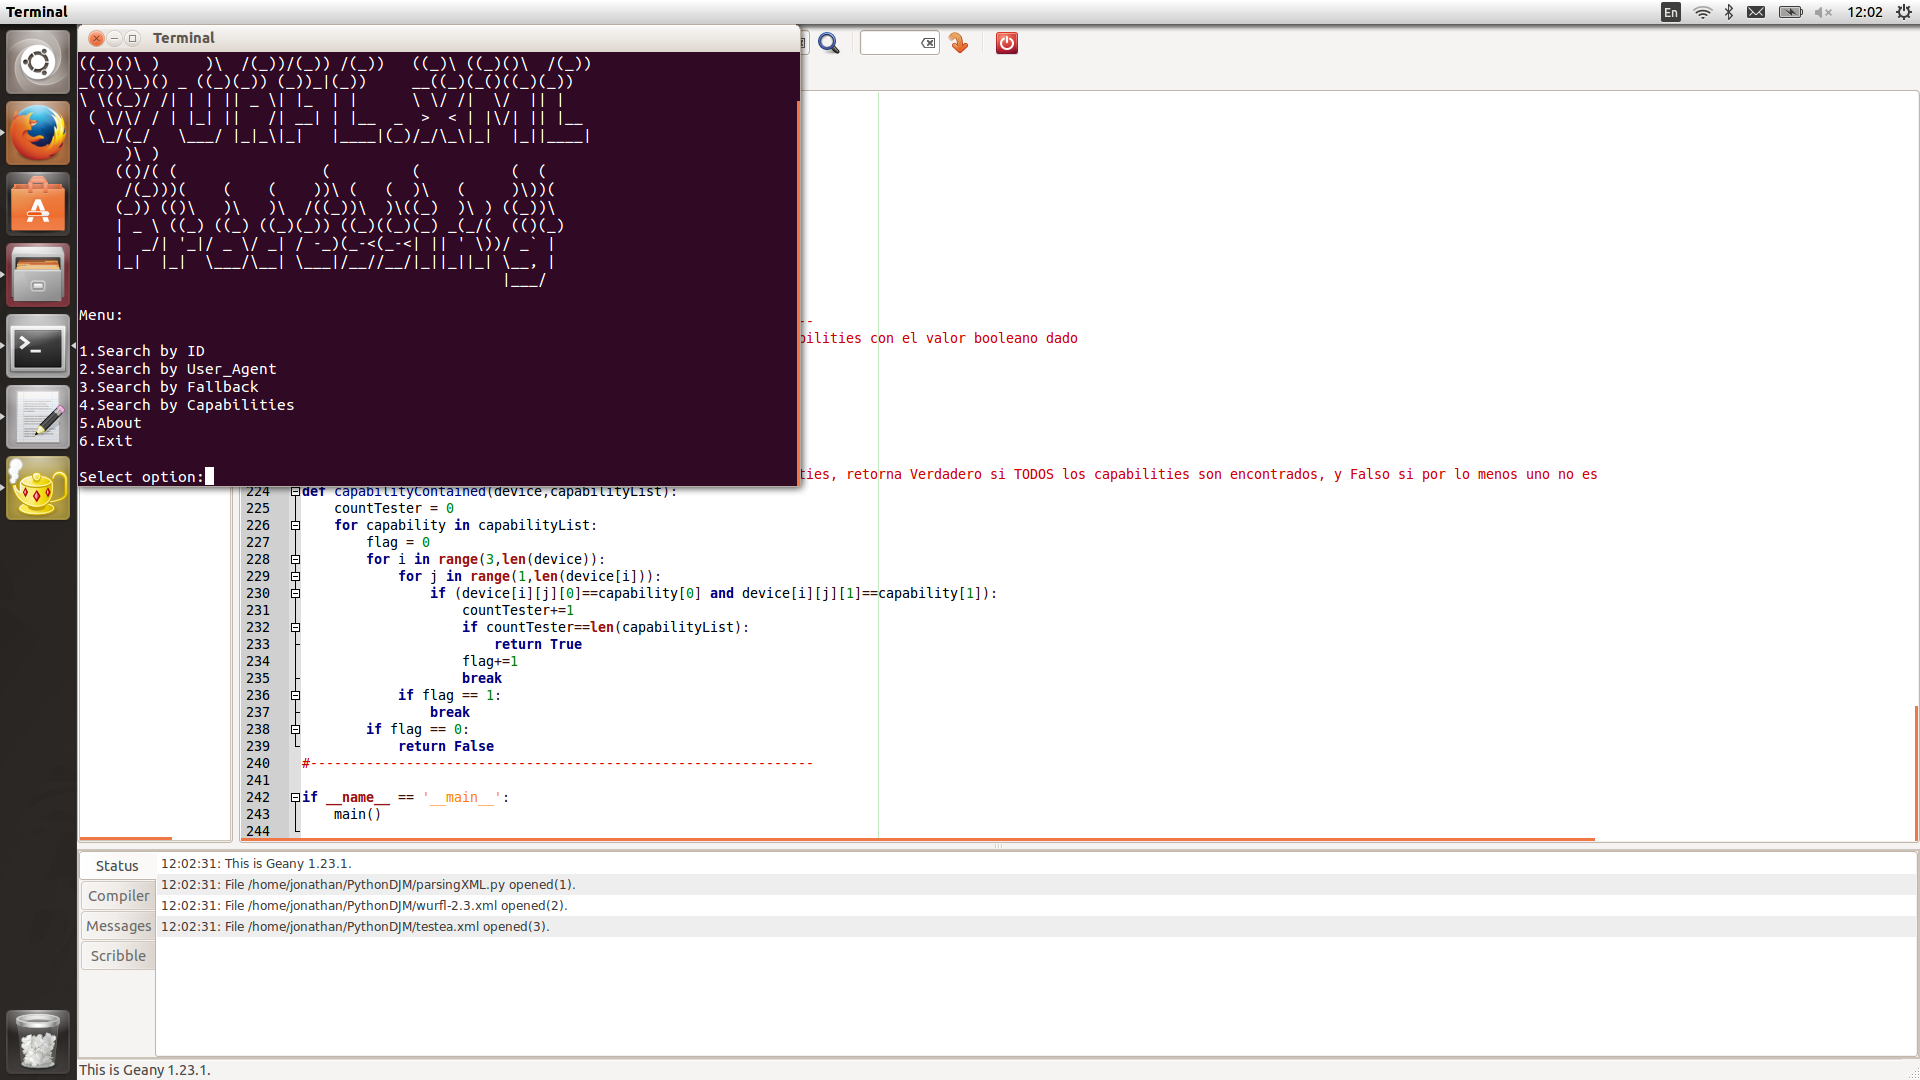
\includegraphics[scale=0.22]{imagenes/sc1.png}
\end{figure}

\begin{figure}
Ingresamos la opcion 1 de buscar por IDs, donde el programa esperara por los valores a buscar (puede contener varias cadenas de caracteres).
\centering
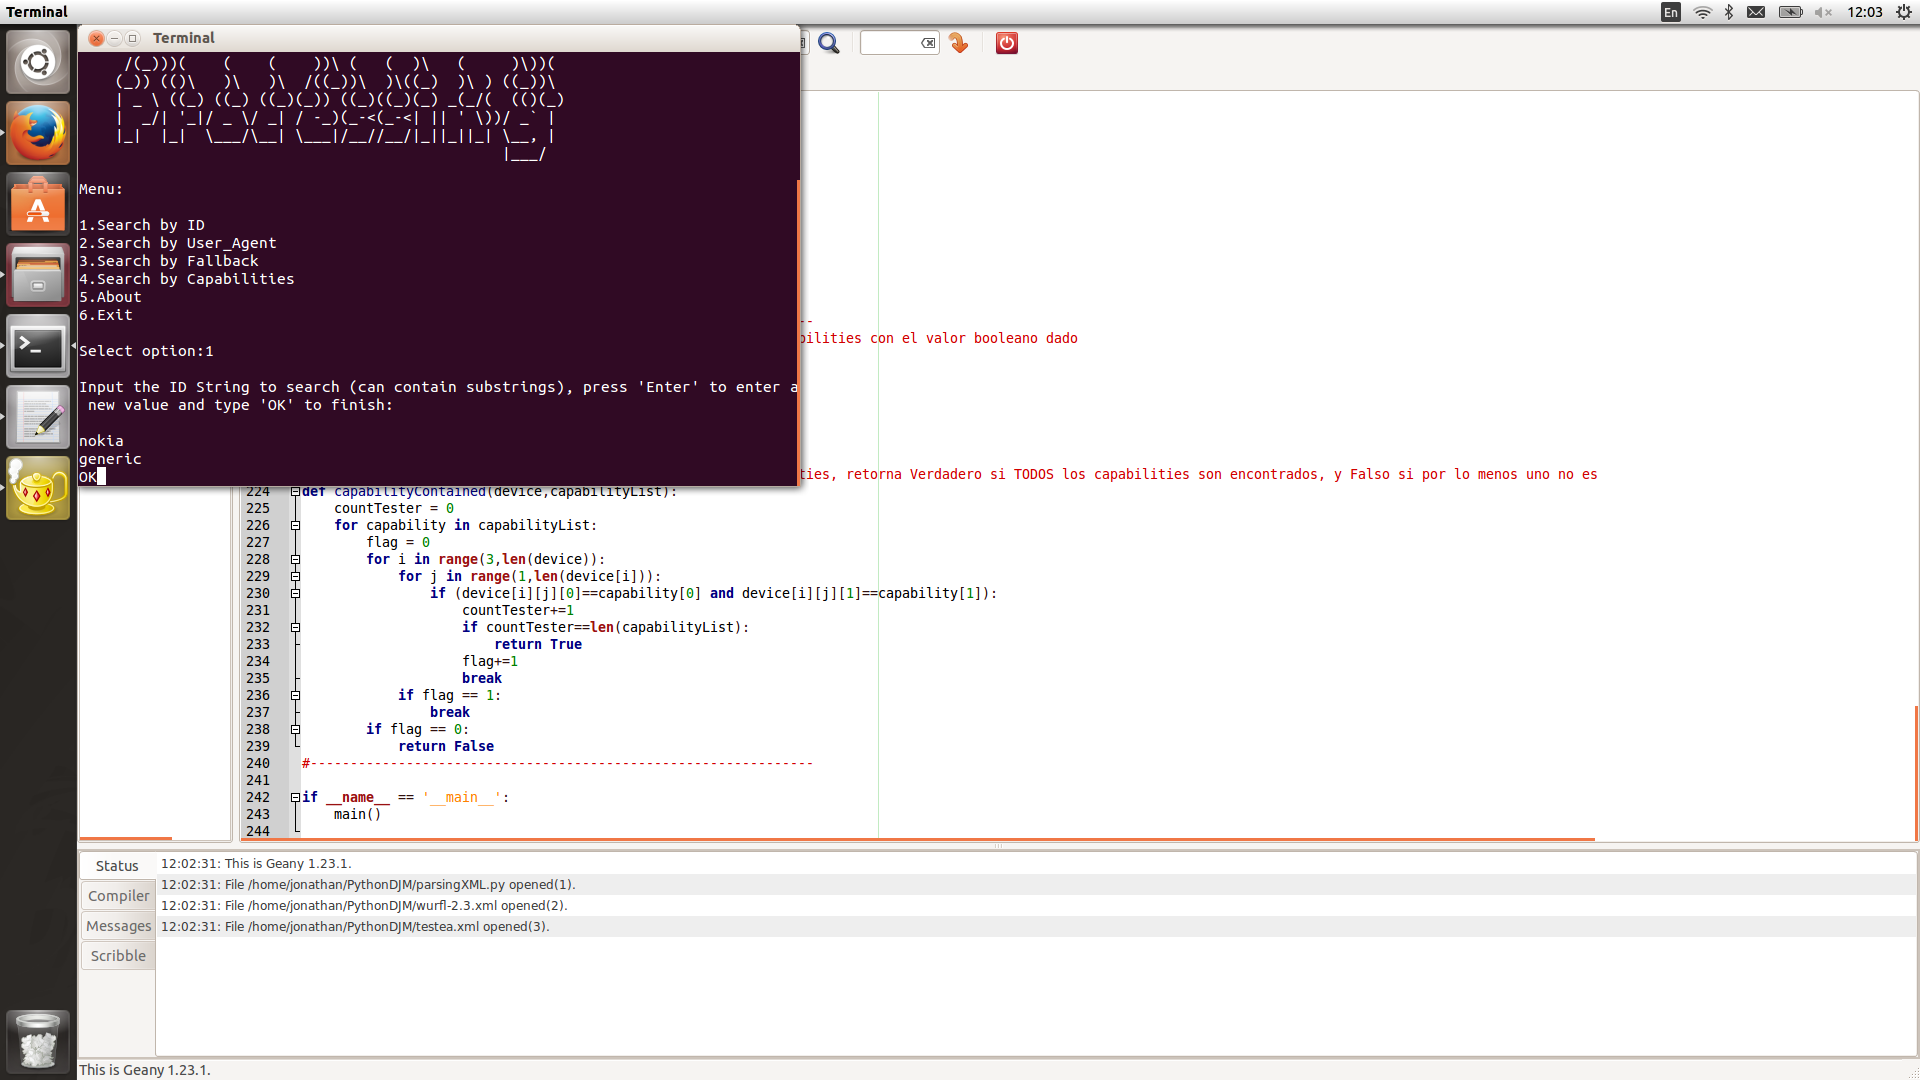
\includegraphics[scale=0.22]{imagenes/sc2.png}
\end{figure}

\begin{figure}
Se ingreso el ID nokia, y a continuacion se muestra lo dispositivos encontrados junto a su numero.
\centering
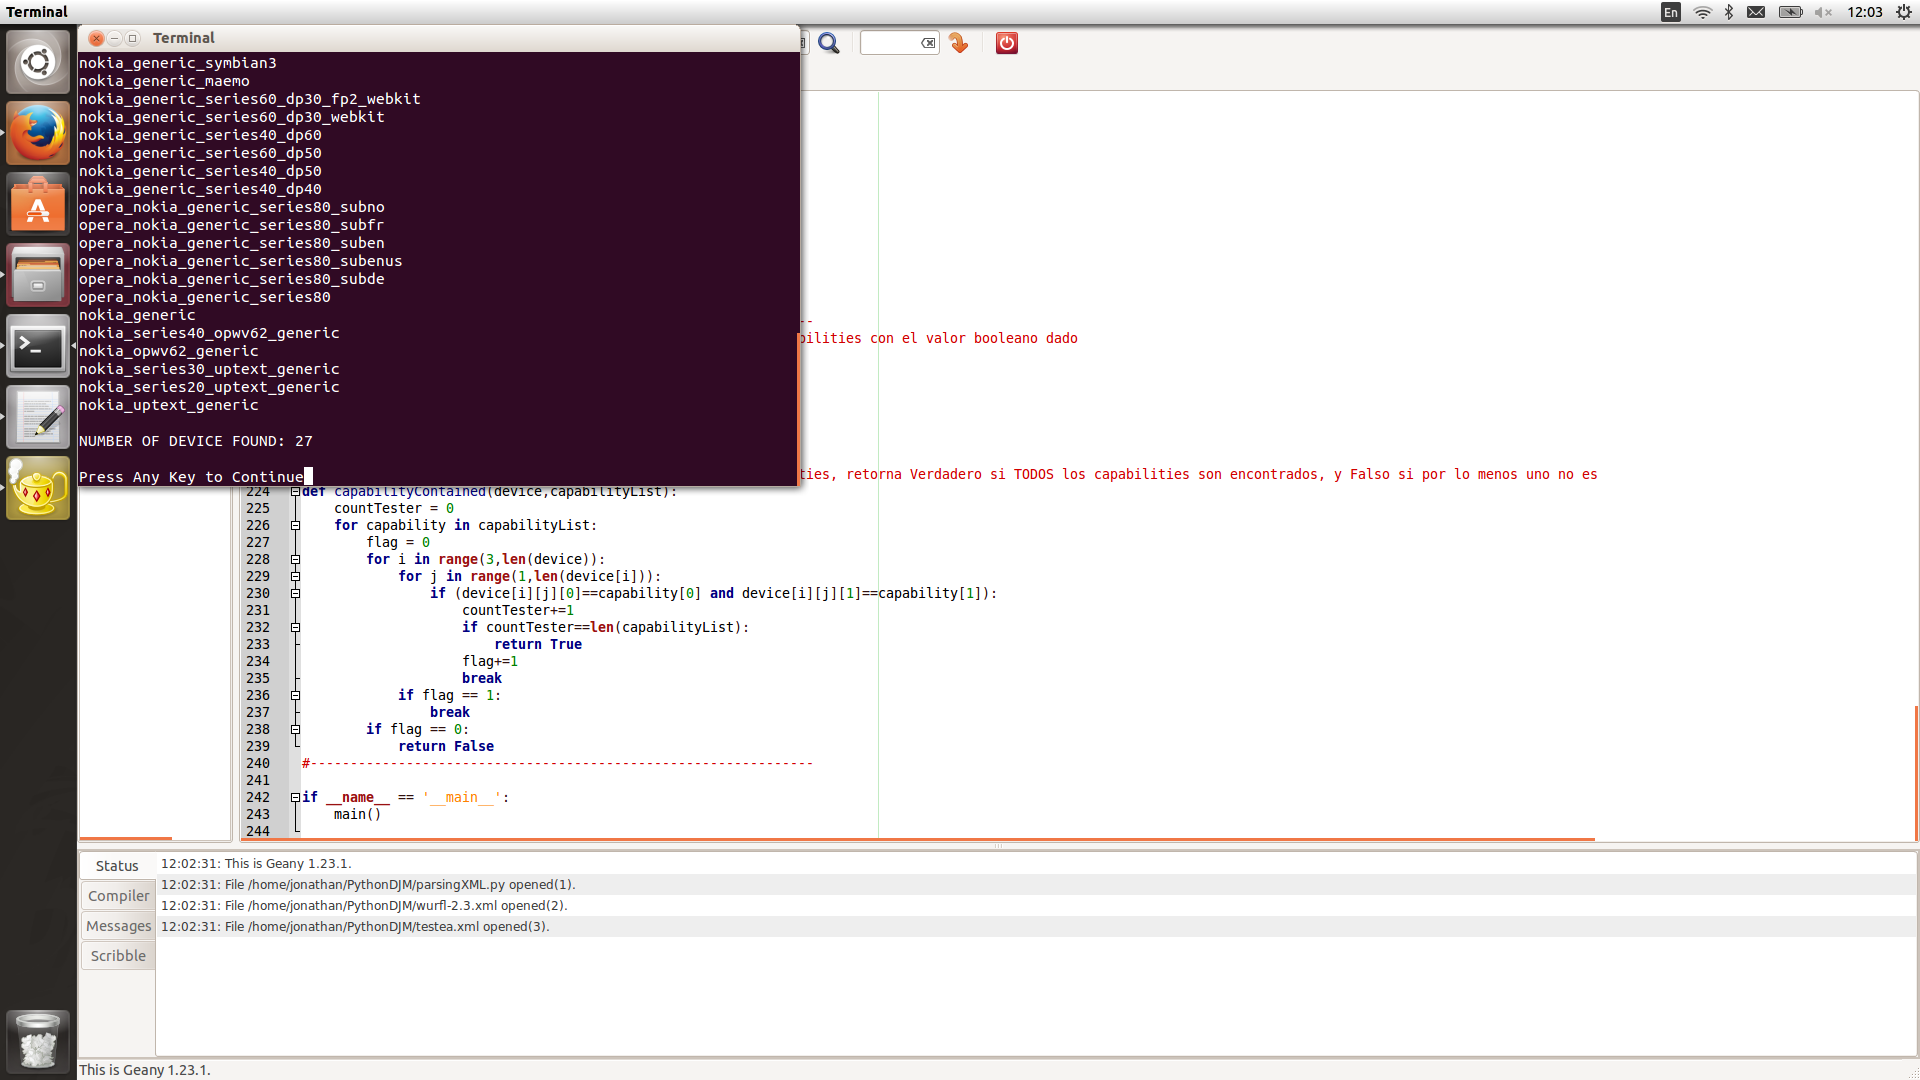
\includegraphics[scale=0.22]{imagenes/sc3.png}
\end{figure}

\begin{figure}
Las opciones de UserAgent y Fallback, son equitativas al ID. En cambio buscar por capabilities es distinto, aqui se podra ingresar mas de una capability a buscar, pero el formato que se pide debe ser el correspondiente, nombre de capability y su valor.
\centering
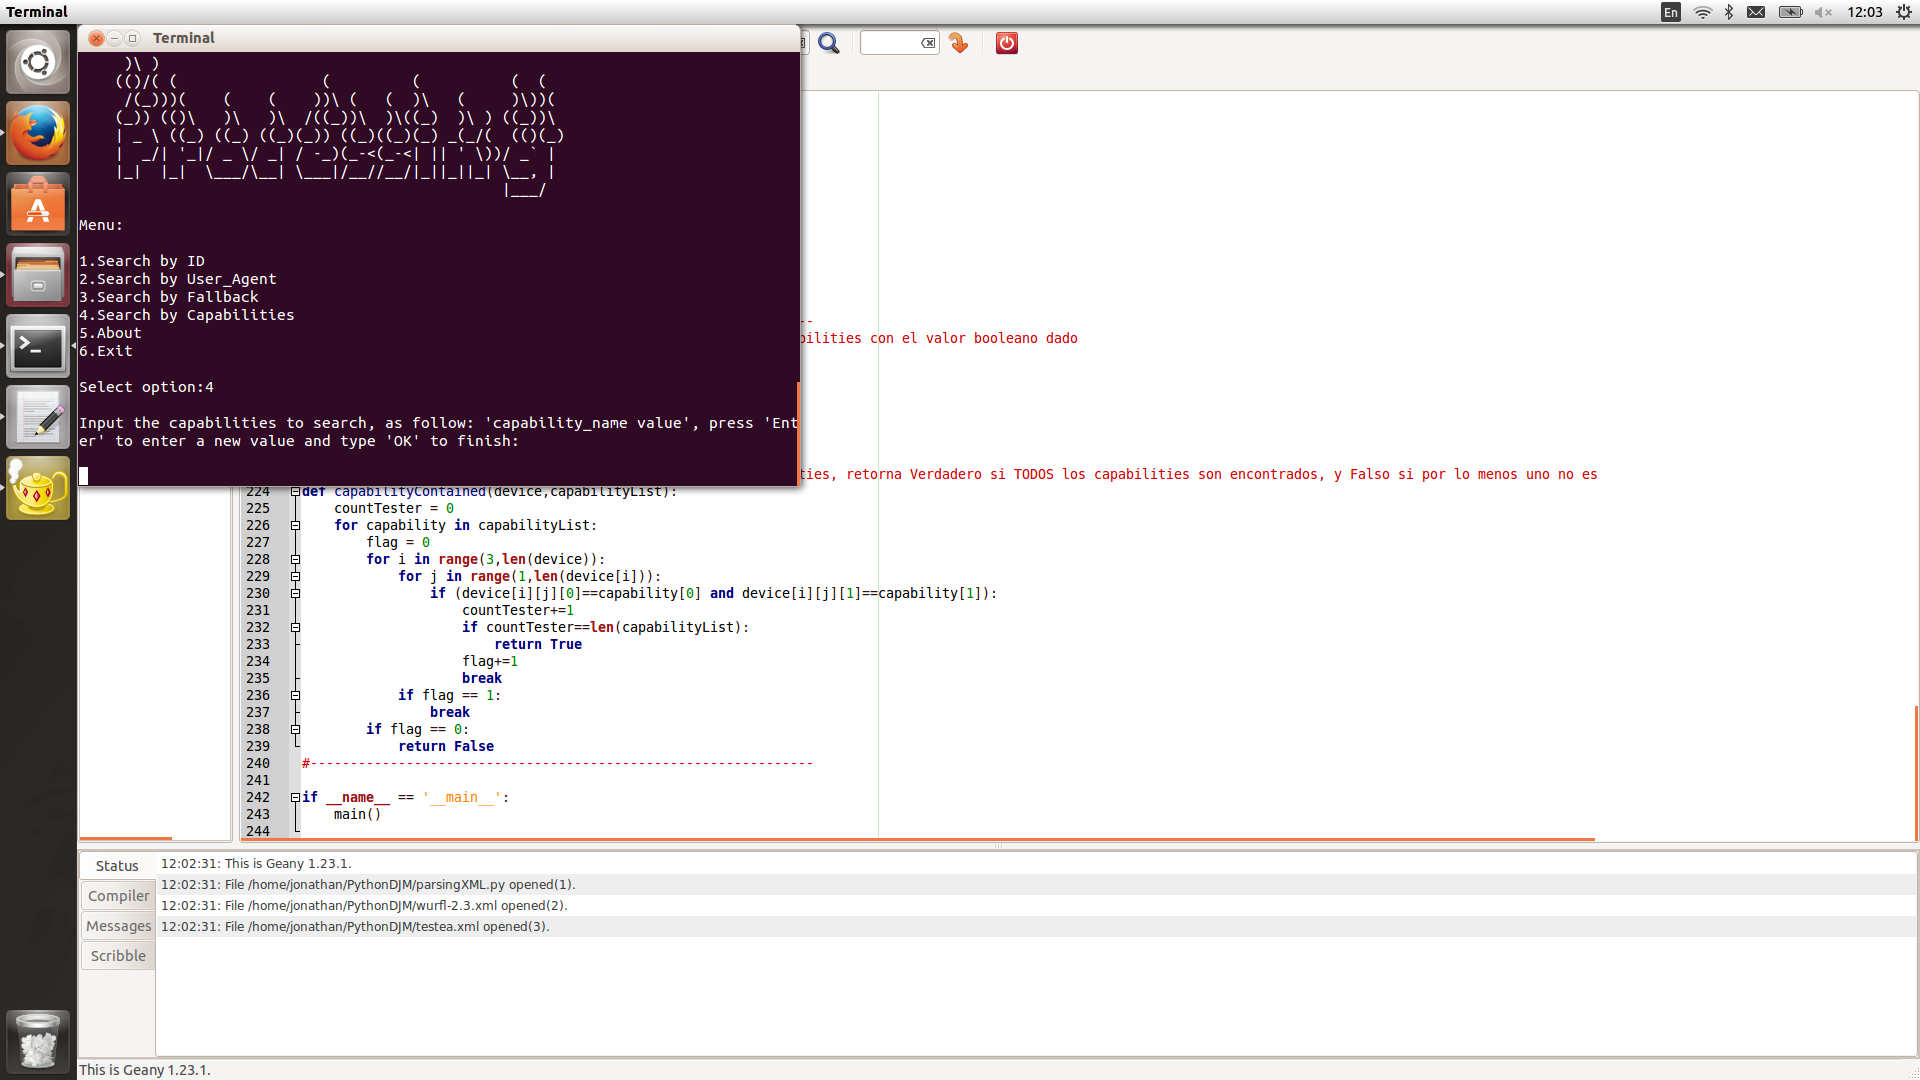
\includegraphics[scale=0.22]{imagenes/sc4.png}
\end{figure}

\begin{figure}
A continuacion buscaremos las capabilities dadas:
\centering
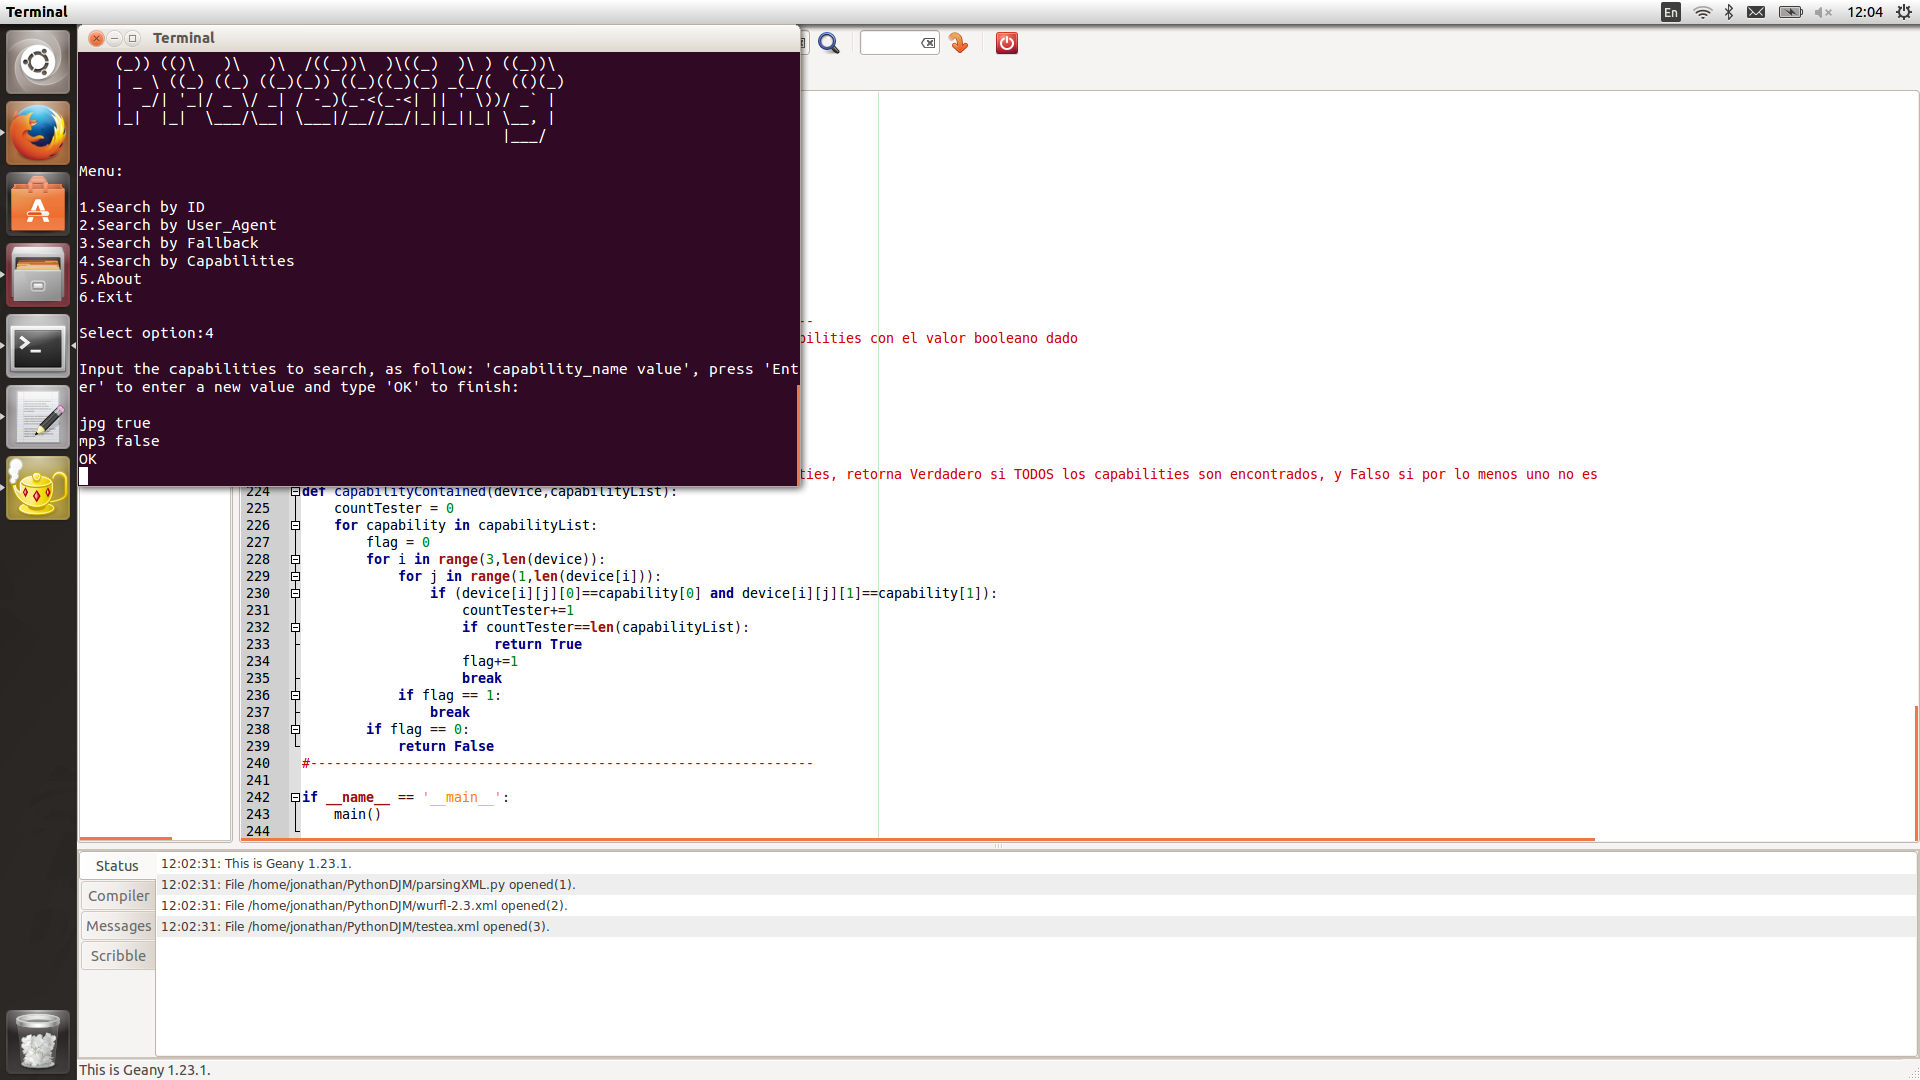
\includegraphics[scale=0.22]{imagenes/sc5.png}
\end{figure}

\begin{figure}
Se muestra el nombre y el numero total de dispositivos encontrados que cumplen con tales capabilities, y los muestra en pantalla.
\centering
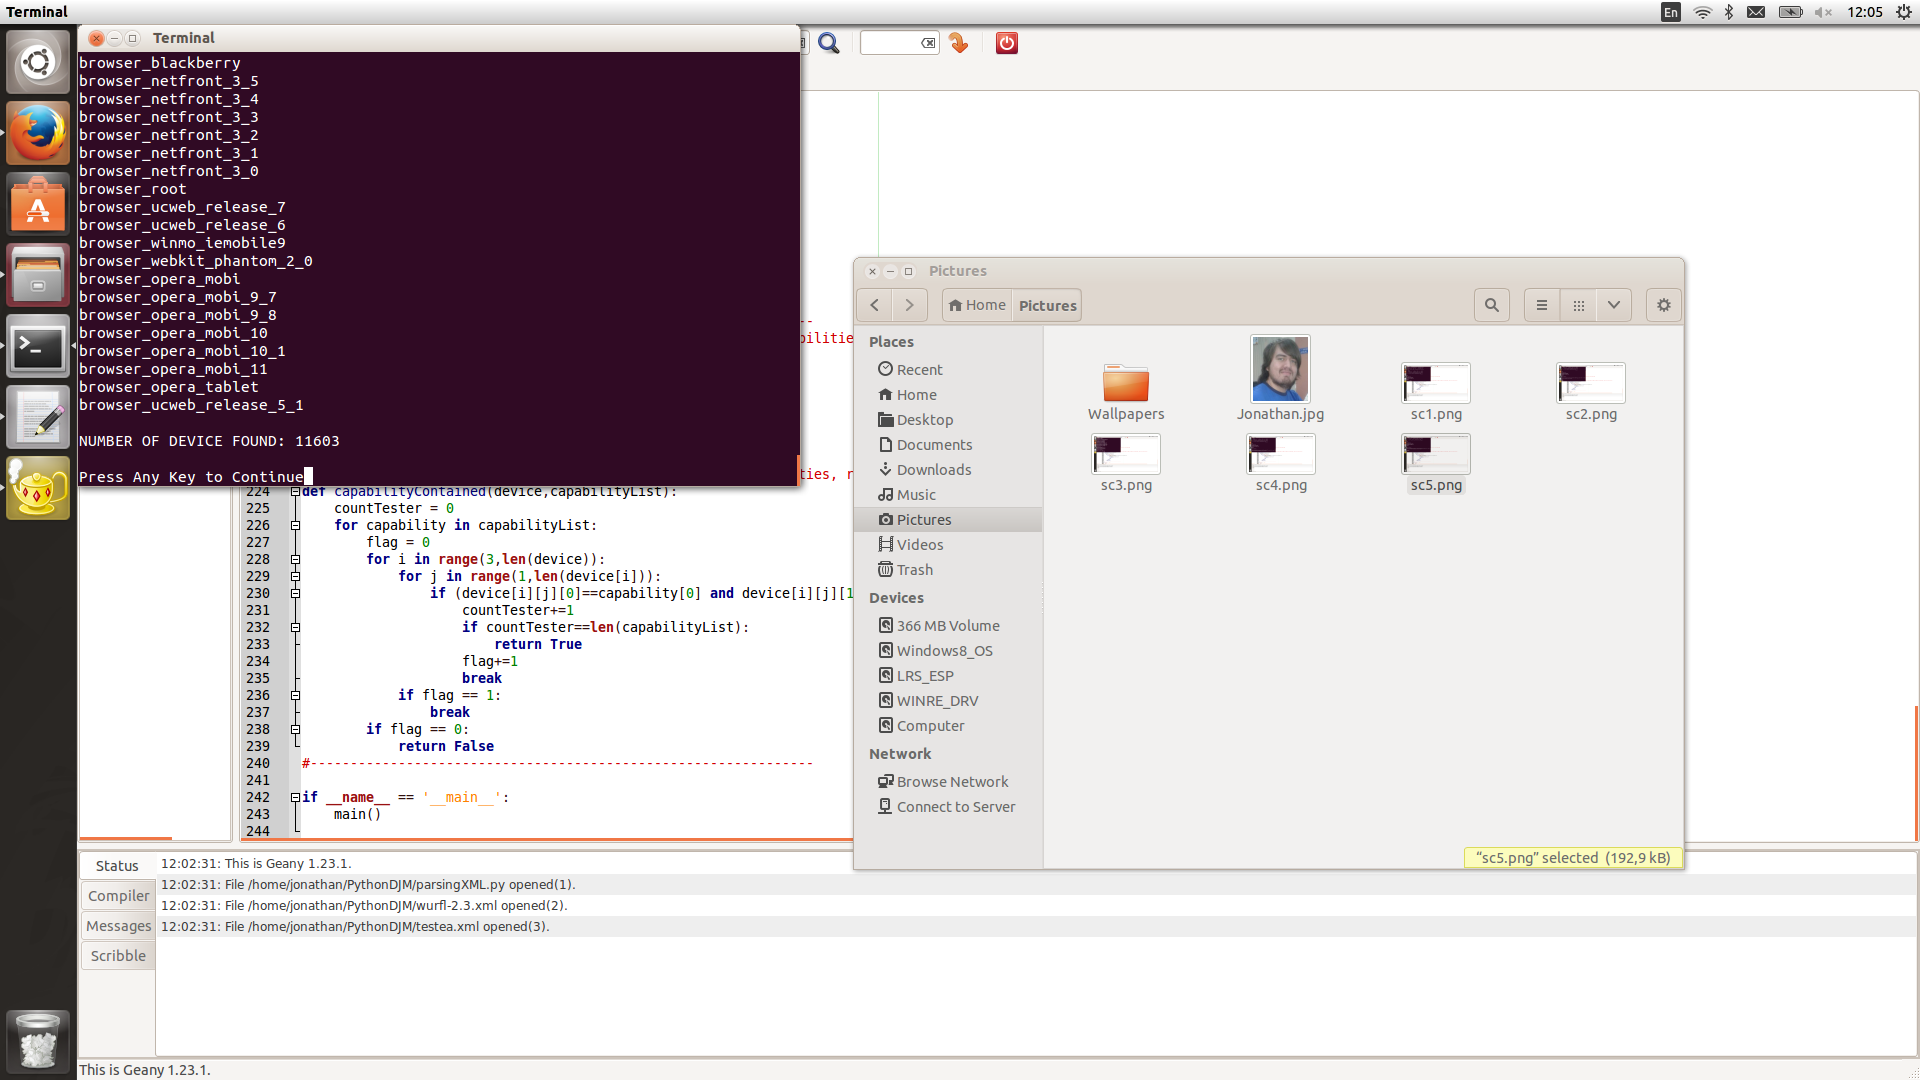
\includegraphics[scale=0.22]{imagenes/sc6.png}
\end{figure}

\begin{figure}
Acerca de muestra a los programadores colaboradores de este proyecto!
\centering
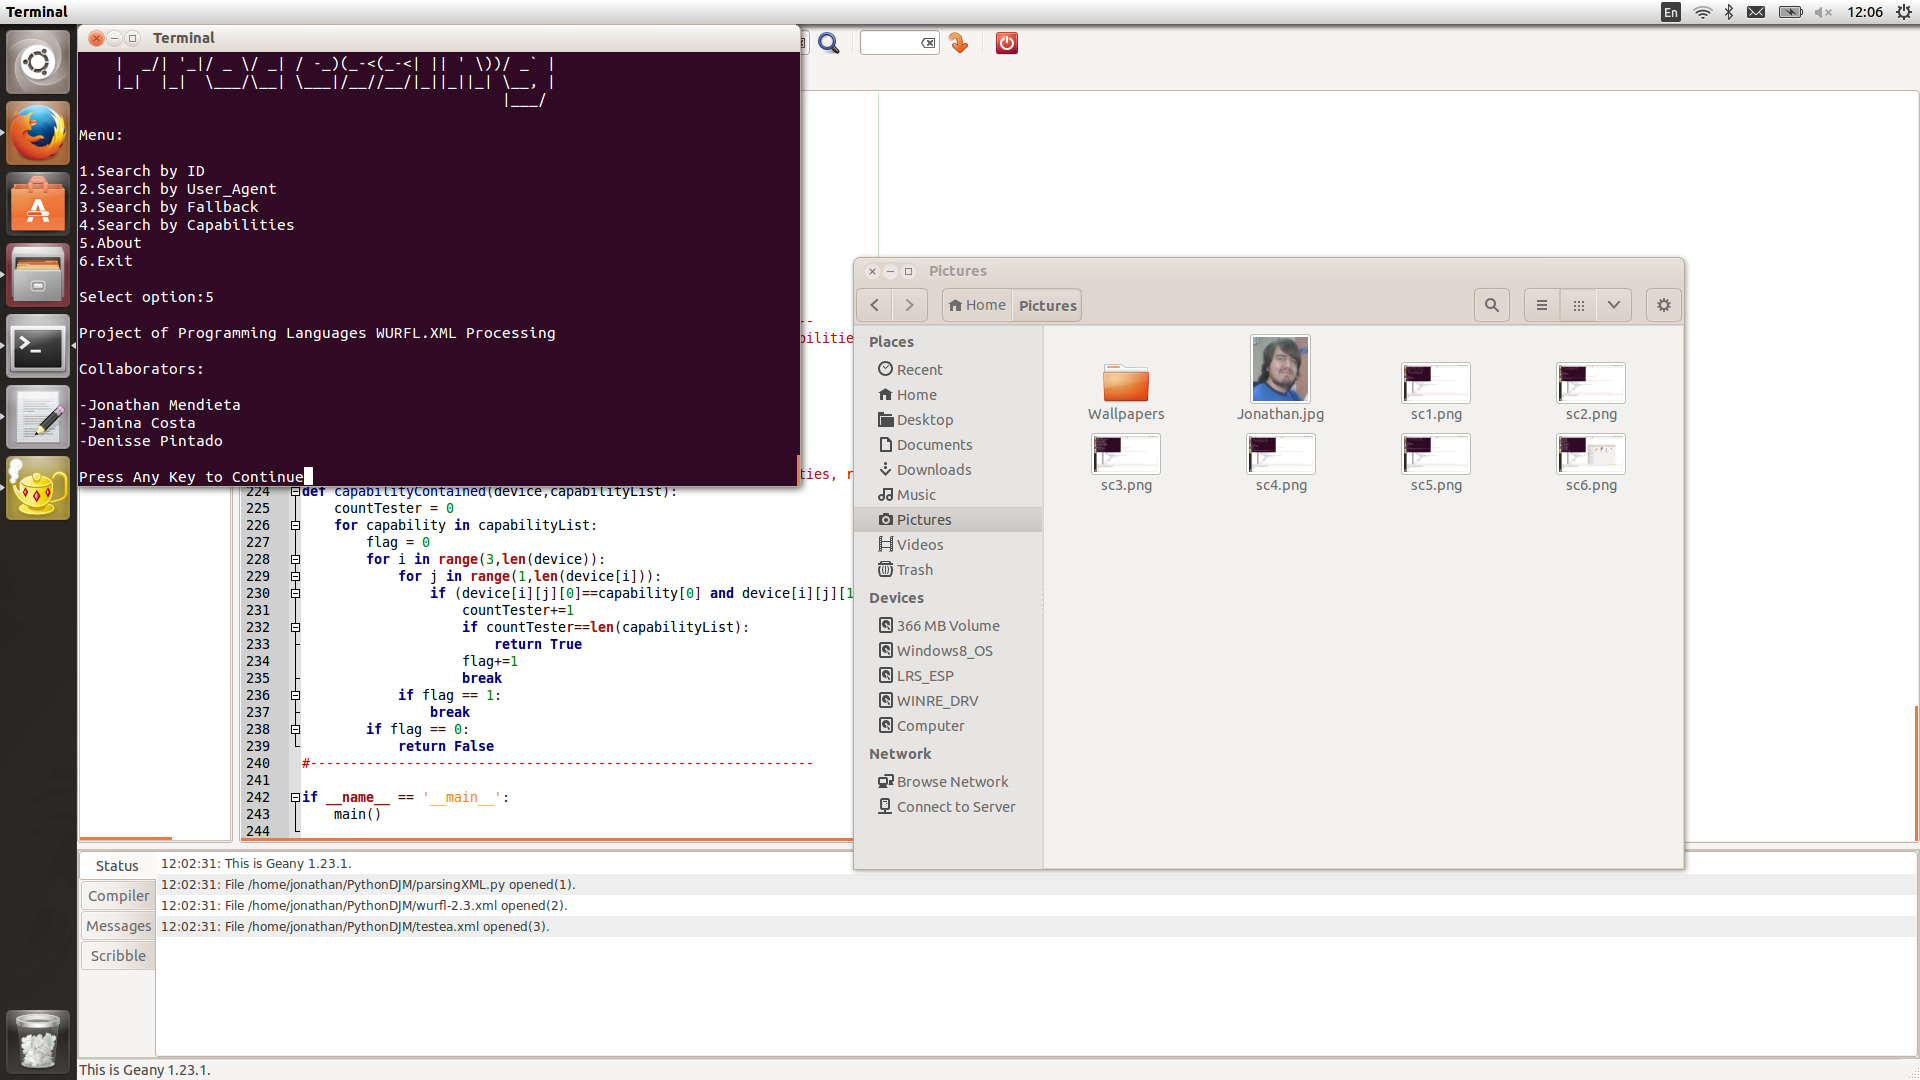
\includegraphics[scale=0.22]{imagenes/sc7.png}
\end{figure}


\section{Ventajas y Desventajas}
VENTAJAS\\
Desarrollo más rápido : Puedes escribir un programa, salvarlo y ejecutarlo. En un lenguaje compilado tienes que pasar por los pasos de compilar y ligar el software, lo cual puede ser un proceso lento.
Multiplataforma : El mismo código funciona en cualquier arquitectura, la única condición es que disponga del intérprete del lenguaje. No es necesario compilar el código una vez para cada arquitectura.\\\\
Flexibilidad : Permite muchas cosas y es faill de aprender
\newline
DESVENTAJAS\\\\
Lentitud : Los programas interpretados son más lentos que los compilados. Sin embargo los programas interpretados suelen ser cortos, en los que la diferencia es inapreciable.

\section{ Conclusiones}
Pyhton es un lenguaje muy sencillo lo unico que se complico al momento de trabajar con el fue la indexacion. Por ser un lenguaje
orientado a objeto, tiene muchas similitudes con Java pero tiene ventajas sobre java muy grandes como la flexibilidad, algo que fue muy notorio al momento de programar. Python ofrece una gran forma de trabajar con listing, al momento de formar el arbol de parseo, se utilizo listas, estas listas contenian las distintas caracteristicas de cada dispositivo.
Esa misma flexibilidad con el manejo de listas, hace a python un lenguaje muy competente, tiene cierta similitud con Haskell en el manejo de las listas y tuplas.

\section{ Recomendaciones}
Una recomendacion en general, es en la construccion del arbol de parseo, porque se debe tener un control en la lectura del archivo. Nuestra algoritmo leia linea por linea y verificaba ciertos patrones, para poder crear la lista que se convertira en el arbol de parseo. Tenemos un modelo unico en cuanto al arbol de parseo, y todo implementamos de acuerdo a cierto modelo. Ademas se debe tener mucho cuidado porque los patrones que comunmente parecen estar en todo el archivo, no son coherentes. Es decir, el archivo tiene dispositivos que cambian en su aspecto.

\end{document}
